\documentclass[11pt,a4paper]{report}
\usepackage[utf8]{inputenc}
\usepackage[T1]{fontenc}
\usepackage{amsmath,amssymb,amsthm}
\usepackage{graphicx}
\usepackage{xcolor}
\usepackage{listings}
\usepackage{algorithm}
\usepackage{algorithmic}
\usepackage{booktabs}
\usepackage{multirow}
\usepackage{longtable}
\usepackage{array}
\usepackage{hyperref}
\usepackage{geometry}
\usepackage{fancyhdr}
\usepackage{enumitem}
\usepackage{titlesec}
\usepackage{tocloft}
\usepackage{caption}
\usepackage{subcaption}
\usepackage{float}
\usepackage{pdflscape}
\usepackage{tikz}
\usetikzlibrary{shapes,arrows,positioning,calc,backgrounds,fit}

% Page geometry
\geometry{
    a4paper,
    left=25mm,
    right=25mm,
    top=30mm,
    bottom=30mm
}

% Color definitions
\definecolor{primaryblue}{RGB}{30,58,138}
\definecolor{secondaryblue}{RGB}{37,99,235}
\definecolor{lightblue}{RGB}{59,130,246}
\definecolor{darkgray}{RGB}{75,85,99}
\definecolor{codebg}{RGB}{245,245,245}

% Section formatting
\titleformat{\chapter}[display]
{\normalfont\huge\bfseries\color{primaryblue}}{\chaptertitlename\ \thechapter}{20pt}{\Huge}
\titleformat{\section}
{\normalfont\Large\bfseries\color{primaryblue}}{\thesection}{1em}{}
\titleformat{\subsection}
{\normalfont\large\bfseries\color{secondaryblue}}{\thesubsection}{1em}{}
\titleformat{\subsubsection}
{\normalfont\normalsize\bfseries\color{lightblue}}{\thesubsubsection}{1em}{}

% Header and footer
\pagestyle{fancy}
\fancyhf{}
\fancyhead[L]{\small\textit{Adaptive Learning System for Higher Education}}
\fancyhead[R]{\small\textit{Implementation Roadmap}}
\fancyfoot[C]{\thepage}
\renewcommand{\headrulewidth}{0.4pt}
\renewcommand{\footrulewidth}{0.4pt}

% Code listings setup
\lstdefinestyle{pythonstyle}{
    language=Python,
    basicstyle=\small\ttfamily,
    backgroundcolor=\color{codebg},
    keywordstyle=\color{primaryblue}\bfseries,
    commentstyle=\color{darkgray}\itshape,
    stringstyle=\color{secondaryblue},
    numbers=left,
    numberstyle=\tiny\color{darkgray},
    stepnumber=1,
    numbersep=5pt,
    breaklines=true,
    frame=single,
    frameround=tttt,
    framexleftmargin=5mm,
    xleftmargin=10mm,
    xrightmargin=5mm,
    captionpos=b
}

\lstset{style=pythonstyle}

% Hyperref setup
\hypersetup{
    colorlinks=true,
    linkcolor=primaryblue,
    filecolor=secondaryblue,
    urlcolor=lightblue,
    citecolor=primaryblue,
    pdftitle={Adaptive Learning System for Higher Education},
    pdfauthor={AI Architecture Team},
    pdfsubject={Implementation Roadmap},
    pdfkeywords={adaptive learning, higher education, AI, pedagogy, IRT}
}

\begin{document}

% Title page
\begin{titlepage}
    \centering
    \vspace*{2cm}
    {\Huge\bfseries\color{primaryblue} Adaptive Learning System\\[0.5cm]
    for Higher Education\\[1cm]}
    \Large{Architecture \& Implementation Roadmap}\\[2cm]
    
    \large{A Comprehensive Framework for AI-Driven\\
    Personalized Learning at University Level}\\[3cm]
    
    \begin{abstract}
    \noindent This document presents a detailed architectural design and implementation roadmap for an adaptive learning system specifically optimized for higher education environments. The system employs a hybrid approach combining Retrieval-Augmented Generation (RAG), cross-encoder reranking, and contextual bandits to deliver personalized micro-learning experiences while optimizing for deep conceptual understanding and knowledge transfer. With a focus on university-level cognitive demands, the framework integrates sophisticated pedagogical strategies, Item Response Theory (IRT) based assessment, and continuous optimization through reinforcement learning. The 12-week implementation plan targets 30\% improvement in problem-solving transfer and 70\% concept retention at 30 days post-instruction.
    \end{abstract}
    
    \vfill
    \today
\end{titlepage}

% Table of contents
\tableofcontents
\newpage

\chapter{Executive Summary}

\section{Strategic Overview}

The recommended approach combines Hybrid RAG with Cross-Encoder Reranking and Contextual Bandits, enhanced with advanced pedagogical tools specifically designed for higher education learners. This architecture addresses the unique cognitive demands of university-level learning while maintaining scalability and continuous improvement capabilities.

\section{Key Recommendations}

\begin{enumerate}[leftmargin=*]
    \item \textbf{Target Audience}: University/college students (ages 18-25+), graduate students, and adult professional learners requiring deep conceptual understanding
    
    \item \textbf{Core Innovation}: Micro-learning constraint engine (2-5 minute chunks) balanced with higher-order thinking assessments using revised Bloom's taxonomy (analyzing, evaluating, creating)
    
    \item \textbf{Pedagogical Focus}: Case-based reasoning, problem-solving scaffolding, conceptual prerequisites mapping, and academic writing support
    
    \item \textbf{Assessment Strategy}: IRT 3PL model calibrated for university-level complexity, with emphasis on open-ended responses and multi-step problem solving
    
    \item \textbf{Data Strategy}: Bootstrap with course syllabi, lecture transcripts, academic papers; leverage existing LMS data for prior knowledge modeling
    
    \item \textbf{Key Differentiator}: Multi-objective reward optimizing for deep learning (conceptual mastery) over surface learning (memorization)
    
    \item \textbf{Risk Mitigation}: Faculty advisory board, academic integrity checks, prerequisite verification, and instructor dashboard for oversight
    
    \item \textbf{Success Metrics}: 
    \begin{itemize}
        \item 30\% improvement in problem-solving transfer
        \item 25\% improvement in concept retention at 30 days
        \item 40\% reduction in time-to-competency
    \end{itemize}
    
    \item \textbf{Investment}: \$150K compute/infrastructure, 4-6 FTEs for 12 weeks, ongoing \$20K/month for inference at scale
\end{enumerate}

\chapter{Architecture Comparison and Selection}

\section{Comparative Analysis}

\begin{table}[H]
\centering
\caption{Architecture Options Comparison}
\label{tab:architecture-comparison}
\begin{tabular}{p{3cm}p{3cm}p{3cm}p{3cm}p{3cm}}
\toprule
\textbf{Aspect} & \textbf{RAG + Rerank} & \textbf{LoRA + RAG} & \textbf{RL/Bandits} & \textbf{Task-Specific} \\
\midrule
\textbf{Components} & Embeddings, VectorDB, Cross-encoder & Base LLM + Adapters & RAG + Bandits & Multiple 7B models \\
\textbf{Setup Cost} & \$30K & \$80K & \$50K & \$120K \\
\textbf{Monthly Cost} & \$10K & \$15K & \$12K & \$25K \\
\textbf{Latency} & 200-400ms & 150-300ms & 250-450ms & 100-200ms \\
\textbf{Cold-Start} & Excellent & Poor & Excellent & Very Poor \\
\textbf{Learning Impact} & Moderate & Moderate-High & \textbf{High} & High \\
\textbf{Team Fit} & Excellent & Good & \textbf{Excellent} & Poor \\
\bottomrule
\end{tabular}
\end{table}

\section{Recommended Architecture}

The optimal solution combines \textbf{Option C (RL/Bandits + RAG)} with elements of Option A (reranking), providing immediate functionality with continuous improvement directly optimized for learning outcomes.

\subsection{System Architecture}

\begin{figure}[H]
\centering
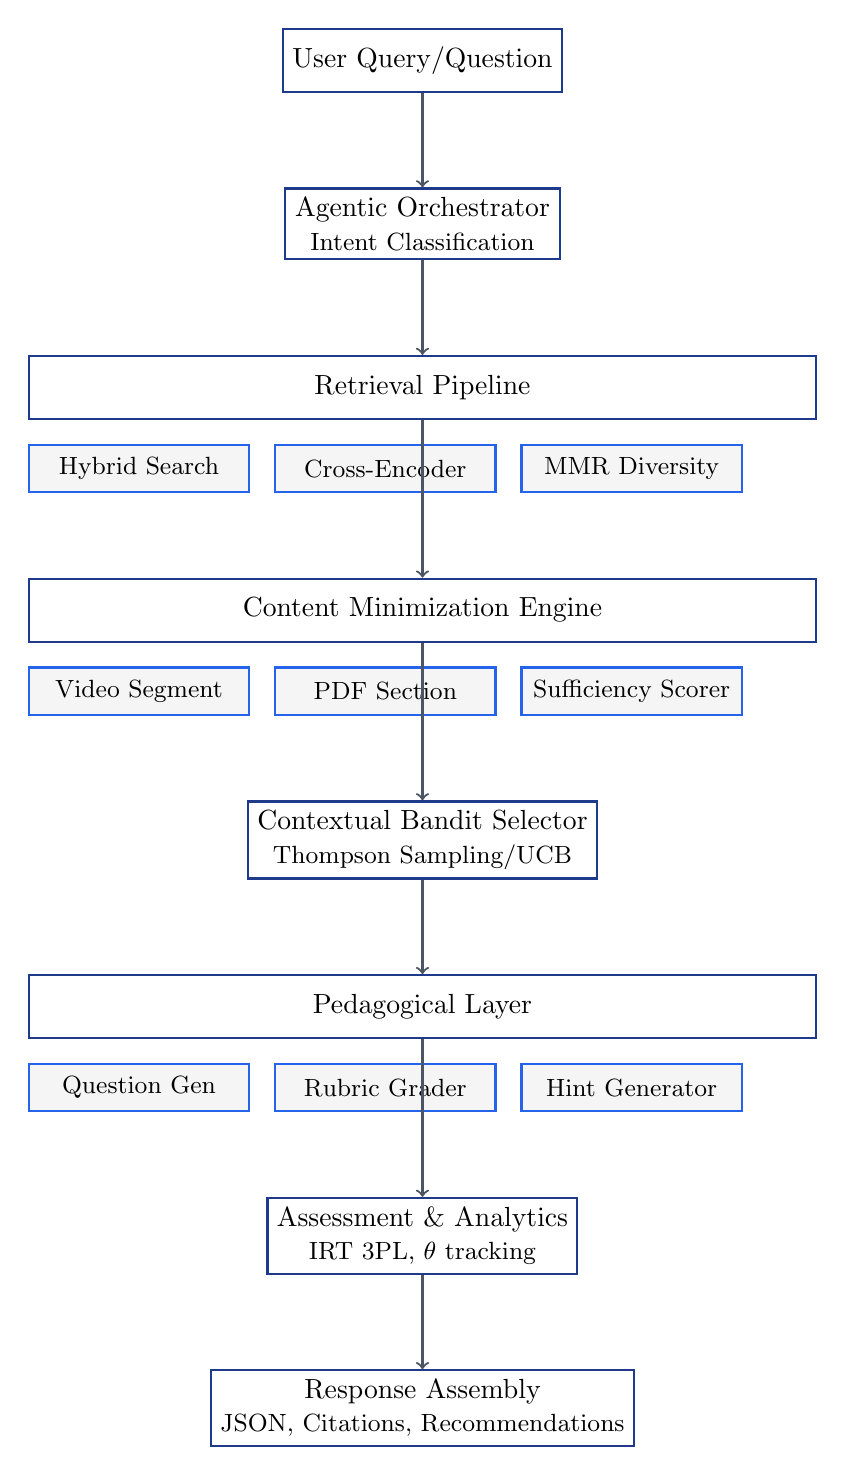
\begin{tikzpicture}[
    node distance=1.2cm,
    box/.style={rectangle, draw=primaryblue, fill=white, thick, minimum width=3.5cm, minimum height=0.8cm, align=center},
    component/.style={rectangle, draw=secondaryblue, fill=codebg, thick, minimum width=2.8cm, minimum height=0.6cm, align=center, font=\small},
    arrow/.style={->, thick, color=darkgray},
    wide/.style={minimum width=10cm}
]

% User Input
\node[box] (input) {User Query/Question};

% Orchestrator
\node[box, below=of input] (orchestrator) {Agentic Orchestrator\\{\small Intent Classification}};

% Retrieval Pipeline
\node[box, wide, below=of orchestrator] (retrieval) {Retrieval Pipeline};
\node[component, below=0.3cm of retrieval.south west, anchor=north west] (hybrid) {Hybrid Search};
\node[component, right=0.3cm of hybrid] (rerank) {Cross-Encoder};
\node[component, right=0.3cm of rerank] (mmr) {MMR Diversity};

% Content Minimization
\node[box, wide, below=2cm of retrieval] (minimize) {Content Minimization Engine};
\node[component, below=0.3cm of minimize.south west, anchor=north west] (video) {Video Segment};
\node[component, right=0.3cm of video] (pdf) {PDF Section};
\node[component, right=0.3cm of pdf] (score) {Sufficiency Scorer};

% Bandit Selector
\node[box, below=2cm of minimize] (bandit) {Contextual Bandit Selector\\{\small Thompson Sampling/UCB}};

% Pedagogical Layer
\node[box, wide, below=of bandit] (pedagogy) {Pedagogical Layer};
\node[component, below=0.3cm of pedagogy.south west, anchor=north west] (question) {Question Gen};
\node[component, right=0.3cm of question] (rubric) {Rubric Grader};
\node[component, right=0.3cm of rubric] (hint) {Hint Generator};

% Assessment Engine
\node[box, below=2cm of pedagogy] (assessment) {Assessment \& Analytics\\{\small IRT 3PL, $\theta$ tracking}};

% Response
\node[box, below=of assessment] (response) {Response Assembly\\{\small JSON, Citations, Recommendations}};

% Arrows
\draw[arrow] (input) -- (orchestrator);
\draw[arrow] (orchestrator) -- (retrieval);
\draw[arrow] (retrieval) -- (minimize);
\draw[arrow] (minimize) -- (bandit);
\draw[arrow] (bandit) -- (pedagogy);
\draw[arrow] (pedagogy) -- (assessment);
\draw[arrow] (assessment) -- (response);

\end{tikzpicture}
\caption{System Architecture for Adaptive Learning}
\label{fig:architecture}
\end{figure}

\chapter{Higher Education Specific Components}

\section{Academic Content Specialization}

\subsection{Research Paper Processing}
\begin{itemize}
    \item Semantic Scholar \& arXiv API integration for peer-reviewed sources
    \item Citation network analysis using PageRank for authority scoring
    \item Structure-aware chunking: Abstract $\rightarrow$ Introduction $\rightarrow$ Methods $\rightarrow$ Results $\rightarrow$ Discussion
    \item Equation and figure extraction with context preservation
\end{itemize}

\subsection{Lecture Material Optimization}
\begin{itemize}
    \item Slide deck analysis with OCR for embedded text extraction
    \item Concept density scoring (technical terms per minute)
    \item Instructor emphasis detection via audio analysis
    \item Synchronized slide-transcript alignment
\end{itemize}

\subsection{Prerequisite and Curriculum Mapping}
\begin{itemize}
    \item Course catalog integration for prerequisite chains
    \item Concept dependency graphs using NLP on syllabi
    \item Adaptive remediation paths for knowledge gaps
    \item Credit hour weighted complexity scoring
\end{itemize}

\section{Advanced Pedagogical Strategies}

\subsection{Higher-Order Thinking Emphasis (Bloom's Revised Taxonomy)}

\begin{table}[H]
\centering
\caption{Higher-Order Thinking Implementation}
\begin{tabular}{lll}
\toprule
\textbf{Level} & \textbf{Cognitive Process} & \textbf{Implementation} \\
\midrule
Analyzing & Differentiate, Organize & Case comparison, Data interpretation \\
Evaluating & Check, Critique & Peer review simulation, Source assessment \\
Creating & Generate, Produce & Research proposals, Solution design \\
\bottomrule
\end{tabular}
\end{table}

\subsection{Cognitive Load Management}

\begin{equation}
CL_{total} = CL_{intrinsic} + CL_{extraneous} + CL_{germane}
\end{equation}

Where:
\begin{itemize}
    \item $CL_{intrinsic}$: Estimated based on concept novelty and prerequisite gaps
    \item $CL_{extraneous}$: Reduced via focused segments and clear presentation
    \item $CL_{germane}$: Optimized through worked examples and scaffolding
\end{itemize}

\section{Assessment Complexity for Higher Education}

\subsection{IRT Model Adaptations}

For university-level assessment, we employ the 3-Parameter Logistic (3PL) model:

\begin{equation}
P(\theta) = c + \frac{1 - c}{1 + e^{-a(\theta - b)}}
\end{equation}

Where:
\begin{itemize}
    \item $\theta$: Student ability parameter
    \item $a$: Item discrimination
    \item $b$: Item difficulty
    \item $c$: Pseudo-guessing parameter
\end{itemize}

\subsection{Learning Gain Measurement}

\begin{equation}
\Delta\theta = \theta_{post} - \theta_{pre}
\end{equation}

\begin{equation}
\text{Normalized Gain} = \frac{\Delta\theta}{3 - \theta_{pre}}
\end{equation}

\chapter{Data Strategy for Higher Education}

\section{Phase 1: Zero-Shot Bootstrap with Academic Sources}

\subsection{LMS Integration}
\begin{enumerate}
    \item Extract existing course materials from Canvas/Blackboard/Moodle
    \item Parse learning objectives, weekly topics, reading assignments from syllabi
    \item Process lecture recordings via WhisperX for concept identification
    \item Utilize course codes, prerequisites, credit hours for complexity scoring
    \item Integrate OpenCourseWare from MIT, Stanford, Coursera
    \item Prioritize faculty-curated resources (weight = 1.5×)
\end{enumerate}

\subsection{Initial Quality Signals}
\begin{itemize}
    \item Course evaluation scores (instructor ratings $>$ 4.0/5)
    \item Textbook adoption rates (widely-used texts = higher quality)
    \item Citation counts for research papers (h-index consideration)
    \item Peer institution usage (cross-reference with consortium data)
\end{itemize}

\section{Phase 2: Rapid Academic Dataset Creation}

\subsection{University-Specific Labeling Protocol}

\begin{table}[H]
\centering
\caption{Difficulty Calibration by Academic Level}
\begin{tabular}{lcc}
\toprule
\textbf{Level} & \textbf{Course Numbers} & \textbf{$\theta$ Range} \\
\midrule
Freshman & 100-200 & [-1, 0] \\
Sophomore/Junior & 300-400 & [0, 1] \\
Senior/Graduate & 500+ & [1, 2] \\
\bottomrule
\end{tabular}
\end{table}

\subsection{Volume Targets (Per Week)}
\begin{itemize}
    \item 500 lecture segment annotations
    \item 300 textbook section mappings
    \item 200 research paper summaries
    \item 100 problem sets with solutions
    \item 50 case studies with rubrics
\end{itemize}

\section{Phase 3: LMS Data Integration}

\subsection{Privacy-Compliant Processing}
\begin{enumerate}
    \item FERPA compliance for all student data
    \item De-identification of all PII
    \item Aggregate-only analytics for small classes ($<20$ students)
    \item Opt-in for individual learning analytics
    \item IRB approval for research uses
\end{enumerate}

\chapter{Metrics and Evaluation Framework}

\section{Learning Outcomes - Primary Success Metrics}

\begin{table}[H]
\centering
\caption{Higher Education Learning Metrics}
\begin{tabular}{p{4cm}p{5cm}p{2cm}p{3cm}}
\toprule
\textbf{Metric} & \textbf{Definition} & \textbf{Target} & \textbf{Measurement} \\
\midrule
Conceptual Mastery ($\Delta\theta$) & $\theta_{post} - \theta_{pre}$ for concepts & $>0.3$ SD & Concept inventories \\
Problem-Solving Transfer & Performance on novel problems & $>30\%$ gain & Capstone assessments \\
Critical Thinking Gain & Argument analysis improvement & $>25\%$ & VALUE rubrics \\
Research Skills & Literature review \& methodology & $>70\%$ & Faculty evaluation \\
Time-to-Competency & Hours to course objectives & $-40\%$ & LMS tracking \\
Long-term Retention & Concept recall at 30 days & $>70\%$ peak & Follow-up tests \\
\bottomrule
\end{tabular}
\end{table}

\section{Content Quality Metrics}

\begin{table}[H]
\centering
\caption{Retrieval and Content Metrics}
\begin{tabular}{lccl}
\toprule
\textbf{Metric} & \textbf{Formula} & \textbf{Target} & \textbf{Frequency} \\
\midrule
nDCG@5 & $\sum_{i=1}^{5} \frac{rel_i}{\log_2(i+1)}$ & $>0.75$ & Weekly \\
Recall@10 & $\frac{|\text{relevant} \cap \text{retrieved}|}{|\text{relevant}|}$ & $>0.85$ & Daily \\
Median Length & Videos (min), PDFs (pages) & $<3$ min, $<2$ pages & Daily \\
Overkill Rate & $\%$ suggestions $>$ threshold & $<10\%$ & Real-time \\
\bottomrule
\end{tabular}
\end{table}

\chapter{Implementation Roadmap}

\section{12-Week Milestone Plan}

\subsection{Milestone 1: RAG Baseline (Weeks 1-2)}

\textbf{Deliverables:}
\begin{itemize}
    \item Hybrid search implementation (BM25 + dense embeddings)
    \item Document chunking pipeline (512 tokens, 128 overlap)
    \item Video segmentation via ASR (2-min chunks)
    \item Basic relevance scoring and length constraints
    \item Offline evaluation harness
\end{itemize}

\textbf{Acceptance Criteria:}
\begin{itemize}
    \item nDCG@5 $>$ 0.65 on test queries
    \item Recall@10 $>$ 0.75
    \item Median resource length $<5$ min (video), $<4$ pages (PDF)
    \item System latency $<600$ms P95
\end{itemize}

\subsection{Milestone 2: Enhanced Retrieval (Weeks 3-4)}

\textbf{Deliverables:}
\begin{itemize}
    \item Cross-encoder reranking (ms-marco-MiniLM)
    \item MMR diversity filtering
    \item Advanced segmentation (scene detection + semantic boundaries)
    \item JSON-structured outputs with metadata
    \item Minimality evaluator with rejection capability
\end{itemize}

\subsection{Milestone 3: Higher Ed Pedagogical Layer V1 (Weeks 5-6)}

\textbf{Deliverables:}
\begin{itemize}
    \item Question generator for higher-order thinking (Analyze/Evaluate/Create)
    \item Case-based problem generator for application scenarios
    \item Rubric grader for open-ended responses and essays
    \item Socratic dialogue system for conceptual exploration
    \item IRT 3PL calibration for university-level complexity
    \item Prior knowledge assessment and prerequisite checking
\end{itemize}

\textbf{Acceptance Criteria:}
\begin{itemize}
    \item Higher-order question ratio $>60\%$ (Bloom's levels 4-6)
    \item Essay grading correlation $>0.75$ with faculty scores
    \item Case problem authenticity $>4.0/5$ (expert review)
    \item IRT parameters stable for 200+ university-level items
\end{itemize}

\subsection{Milestone 4: Adaptive Selection via Bandits (Weeks 7-8)}

\textbf{Deliverables:}
\begin{itemize}
    \item Thompson sampling for content selection
    \item Multi-objective reward function
    \item Off-policy evaluation framework
    \item Exploration bonus for new content
    \item Safety constraints (max length, min relevance)
\end{itemize}

\subsection{Milestone 5: Fine-Tuning Enhancement (Weeks 9-10)}

\textbf{Deliverables:}
\begin{itemize}
    \item LoRA adapter for question generation
    \item Distractor generator fine-tune
    \item Style adapter for explanations
    \item Model versioning and rollback system
    \item Performance comparison report
\end{itemize}

\subsection{Milestone 6: Production Hardening (Weeks 11-12)}

\textbf{Deliverables:}
\begin{itemize}
    \item Safety filters and guardrails
    \item Bias detection and mitigation
    \item FERPA/GDPR compliance audit
    \item Monitoring dashboards (Grafana/Datadog)
    \item Continuous calibration pipeline
    \item Educator oversight interface
\end{itemize}

\chapter{Reinforcement Learning Design}

\section{Reward Function for Higher Education}

\begin{lstlisting}[caption={Multi-objective Reward Function for University Learning},label={lst:reward}]
def calculate_reward_higher_ed(state, action, outcome):
    """
    Multi-objective reward for university-level content selection
    Prioritizes deep learning, conceptual understanding, and transfer
    """
    
    # Deep Learning Component (35% weight)
    concept_mastery_reward = 0.35 * outcome['concept_mastery']
    
    # Transfer Learning (25% weight)
    transfer_reward = 0.25 * outcome['transfer_score']
    
    # Cognitive Efficiency (15% weight)
    efficiency = 1 - (outcome['time_spent'] / 
                     (action['estimated_duration'] * 2))
    efficiency_reward = 0.15 * np.clip(efficiency, -0.5, 1)
    
    # Metacognitive Development (10% weight)
    metacog_reward = 0.1 * outcome['self_explanation_quality']
    
    # Academic Progress (10% weight)
    progress_reward = 0.1 * outcome['delta_theta'] / 0.3
    
    # Zone of Proximal Development (5% weight)
    zpd_distance = abs(action['cognitive_level'] - 
                      (state['ability_level'] + 1))
    if zpd_distance <= 1:
        challenge_reward = 0.05
    else:
        challenge_reward = -0.05 * zpd_distance
    
    # Penalties
    penalties = 0
    
    # Prerequisite violation
    if action['prerequisite_alignment'] < 0.5:
        penalties -= 0.5 * (1 - action['prerequisite_alignment'])
    
    # Cognitive overload
    if action['cognitive_level'] > state['ability_level'] + 2:
        penalties -= 0.3
    
    # Surface learning penalty
    if outcome['concept_mastery'] < 0.3 and outcome['completion'] > 0.8:
        penalties -= 0.2
    
    # Academic integrity risk
    if action.get('integrity_risk', 0) > 0.3:
        penalties -= 1.0
    
    total_reward = (concept_mastery_reward + transfer_reward + 
                   efficiency_reward + metacog_reward + 
                   progress_reward + challenge_reward + penalties)
    
    return total_reward
\end{lstlisting}

\section{Contextual Bandit Algorithm}

\begin{algorithm}
\caption{Academic Thompson Sampling}
\label{alg:thompson}
\begin{algorithmic}[1]
\STATE Initialize resource quality priors $\alpha, \beta \sim \text{Beta}(1,1)$
\STATE Initialize concept coverage matrix $C \in \mathbb{R}^{n \times m}$
\STATE Initialize prerequisite graph $G = (V, E)$

\WHILE{student session active}
    \STATE Observe student state $s$ = \{ability $\theta$, mastered concepts, course\}
    \STATE Check prerequisites: $E_{eligible} = \{r : \text{prereqs}(r) \subseteq s_{mastered}\}$
    \STATE Sample quality: $q_r \sim \text{Beta}(\alpha_r, \beta_r)$ for $r \in E_{eligible}$
    \STATE Compute course alignment: $a_r = \text{alignment}(r, s_{course})$
    \STATE Compute cognitive match: $m_r = 1 - |\text{level}(r) - (\theta + 1)|/6$
    \STATE Score resources: $score_r = 0.4q_r + 0.3a_r + 0.2m_r + 0.1\epsilon$
    \STATE Select resource: $r^* = \arg\max_{r \in E_{eligible}} score_r$
    \STATE Observe outcome: concept mastery, transfer score, time spent
    \STATE Update posteriors: $\alpha_{r^*}, \beta_{r^*}$ based on reward
\ENDWHILE
\end{algorithmic}
\end{algorithm}

\section{Off-Policy Evaluation}

For safe deployment, we employ Inverse Propensity Scoring (IPS) with self-normalization:

\begin{equation}
\hat{V}_{\text{SNIPS}}(\pi_{new}) = \frac{\sum_{i=1}^n w_i r_i}{\sum_{i=1}^n w_i}
\end{equation}

Where $w_i = \frac{\pi_{new}(a_i|s_i)}{\pi_{old}(a_i|s_i)}$ is the importance weight.

\chapter{Higher Education Implementation Considerations}

\section{Integration with University Systems}

\subsection{LMS Integration Requirements}
\begin{itemize}
    \item \textbf{Canvas/Blackboard/Moodle APIs}: Real-time grade sync, assignment submission, discussion forum mining
    \item \textbf{Student Information System (SIS)}: Course enrollment, prerequisite verification, academic standing
    \item \textbf{Library Systems}: Access to academic databases, journal subscriptions, citation management
    \item \textbf{Lecture Capture Platforms}: Panopto, Zoom, Echo360 integration for video processing
    \item \textbf{Academic Calendar Sync}: Adjust pacing based on semester schedule, exam periods
\end{itemize}

\subsection{Faculty Adoption Strategy}

\begin{table}[H]
\centering
\caption{Phased Faculty Adoption Plan}
\begin{tabular}{llp{6cm}}
\toprule
\textbf{Phase} & \textbf{Timeline} & \textbf{Activities} \\
\midrule
Early Adopters & Weeks 1-4 & Recruit 5-10 innovative instructors, white-glove onboarding, co-design features \\
Department Pilots & Weeks 5-8 & Expand to 2-3 departments, create discipline templates, faculty workshops \\
Campus Rollout & Weeks 9-12 & Institution-wide availability, self-service onboarding, peer mentorship \\
\bottomrule
\end{tabular}
\end{table}

\section{Discipline-Specific Customizations}

\subsection{STEM Fields}
\begin{itemize}
    \item LaTeX rendering for mathematical notation
    \item Code execution environments (Jupyter, R Studio)
    \item Virtual lab simulations
    \item Dataset access for statistics/data science
    \item Engineering design tool integration
\end{itemize}

\subsection{Liberal Arts \& Humanities}
\begin{itemize}
    \item Primary source document analysis
    \item Annotation and close reading tools
    \item Multimedia essay support
    \item Foreign language pronunciation
    \item Creative portfolio showcases
\end{itemize}

\subsection{Professional Programs}
\begin{itemize}
    \item Case study libraries (Business, Law, Medicine)
    \item Clinical simulation scenarios
    \item Industry certification alignment
    \item Practicum/internship integration
    \item Professional network connections
\end{itemize}

\section{At-Risk Student Identification}

\begin{lstlisting}[caption={At-Risk Student Detection Algorithm},label={lst:atrisk}]
def identify_at_risk_students(student_metrics):
    risk_factors = {
        'low_engagement': student_metrics['login_frequency'] < 2/week,
        'falling_behind': student_metrics['content_progress'] < 
                         0.7 * expected_progress,
        'struggling': student_metrics['avg_attempt_score'] < 0.6,
        'prerequisite_gaps': len(student_metrics['missing_prereqs']) > 2,
        'time_management': student_metrics['cramming_ratio'] > 0.5
    }
    
    risk_score = sum(risk_factors.values()) / len(risk_factors)
    
    if risk_score > 0.6:
        trigger_interventions(student_id, risk_factors)
    
    return risk_score, risk_factors
\end{lstlisting}

\section{Scalability for Large Enrollments}

\begin{table}[H]
\centering
\caption{Performance Targets by Class Size}
\begin{tabular}{lccc}
\toprule
\textbf{Class Size} & \textbf{Response Time} & \textbf{Concurrent Users} & \textbf{Resource Pool} \\
\midrule
Seminar ($<20$) & $<200$ms & 20 & Shared tier \\
Regular (20-100) & $<300$ms & 100 & Dedicated pod \\
Large (100-500) & $<400$ms & 200 & Scaled cluster \\
MOOC (500+) & $<500$ms & 1000+ & CDN + edge cache \\
\bottomrule
\end{tabular}
\end{table}

\chapter{Risk Analysis and Mitigation}

\section{Technical Risks}

\begin{longtable}{p{3cm}p{2cm}p{2cm}p{6cm}}
\caption{Technical Risk Assessment and Mitigation Strategies} \\
\toprule
\textbf{Risk} & \textbf{Impact} & \textbf{Probability} & \textbf{Mitigation} \\
\midrule
\endfirsthead
\multicolumn{4}{c}{\tablename\ \thetable\ -- \textit{Continued from previous page}} \\
\toprule
\textbf{Risk} & \textbf{Impact} & \textbf{Probability} & \textbf{Mitigation} \\
\midrule
\endhead
\midrule
\multicolumn{4}{r}{\textit{Continued on next page}} \\
\endfoot
\bottomrule
\endlastfoot

Cold-start content & High & High & ASR transcripts + semantic similarity + teacher validation \\
Hallucination & High & Medium & Retrieval grounding + citation requirement + fact-checking \\
Over-long resources & Medium & High & Hard caps + segment ranking + coverage-per-minute metric \\
IRT parameter drift & Medium & Medium & Weekly recalibration + anchor items + drift detection \\
Bandit exploration & Medium & Low & Safety constraints + minimum exploration + off-policy eval \\
\end{longtable}

\section{Data and Privacy Risks}

\begin{itemize}
    \item \textbf{FERPA Compliance}: Implement strict data access controls, anonymization protocols, and parent access portals
    \item \textbf{Academic Integrity}: Develop plagiarism detection, response pattern analysis, and proctoring integration
    \item \textbf{Bias Mitigation}: Regular demographic parity audits, fairness constraints in optimization, diverse training data
\end{itemize}

\chapter{First 14 Days Implementation Plan}

\section{Days 1-3: Infrastructure Setup}
\begin{itemize}
    \item[$\square$] Provision GPU instances for embeddings and reranking
    \item[$\square$] Set up vector database (Pinecone/Weaviate/Qdrant)
    \item[$\square$] Configure experiment tracking (MLflow/W\&B)
    \item[$\square$] Create data versioning system (DVC)
    \item[$\square$] Initialize git repos and CI/CD pipeline
\end{itemize}

\section{Days 4-6: Data Preparation}
\begin{itemize}
    \item[$\square$] Extract and analyze existing Q\&A/assessment data
    \item[$\square$] Create labeling interface for query-resource relevance
    \item[$\square$] Begin ASR transcription of video library (WhisperX)
    \item[$\square$] Design evaluation query set (diverse topics, difficulties)
    \item[$\square$] Establish inter-rater agreement protocol
\end{itemize}

\section{Days 7-9: RAG Baseline Implementation}
\begin{itemize}
    \item[$\square$] Implement document chunking pipeline (text + PDF)
    \item[$\square$] Create video segmentation via ASR timestamps
    \item[$\square$] Build hybrid search (BM25 + dense embeddings)
    \item[$\square$] Add length constraints and filtering
    \item[$\square$] Create JSON output formatting
\end{itemize}

\section{Days 10-11: Evaluation Framework}
\begin{itemize}
    \item[$\square$] Implement nDCG, Recall, Coverage metrics
    \item[$\square$] Create minimality measurements
    \item[$\square$] Build latency profiling tools
    \item[$\square$] Set up offline evaluation harness
    \item[$\square$] Design red team test cases
\end{itemize}

\section{Days 12-13: Initial Testing}
\begin{itemize}
    \item[$\square$] Run baseline evaluation on 100 queries
    \item[$\square$] Conduct latency and scale testing
    \item[$\square$] Perform failure mode analysis
    \item[$\square$] Teacher review of top recommendations
    \item[$\square$] Document findings and pain points
\end{itemize}

\section{Day 14: Milestone 1 Review}
\begin{itemize}
    \item[$\square$] Compile metrics dashboard
    \item[$\square$] Present results to stakeholders
    \item[$\square$] Gather feedback on quality
    \item[$\square$] Refine success criteria for M2
    \item[$\square$] Make go/no-go decision
\end{itemize}

\chapter{Conclusions and Recommendations}

\section{Key Success Factors}

\begin{enumerate}
    \item \textbf{Deep Learning Focus}: The system prioritizes conceptual understanding and transfer capability over memorization, using sophisticated assessment methods (IRT 3PL, open-ended rubrics) to measure true comprehension.
    
    \item \textbf{Academic Rigor}: Integration with research papers, peer-reviewed sources, and university-level materials ensures content meets the intellectual demands of higher education while respecting cognitive load limits.
    
    \item \textbf{Faculty Partnership}: Rather than replacing instructors, the system augments their capabilities through co-creation tools, oversight dashboards, and alignment with course objectives and academic governance.
    
    \item \textbf{Student Development}: Beyond content delivery, the system fosters metacognitive skills, critical thinking, and self-directed learning capabilities essential for university success and lifelong learning.
    
    \item \textbf{Institutional Integration}: Deep integration with existing university infrastructure (LMS, SIS, library systems) ensures seamless adoption and value realization within the academic ecosystem.
\end{enumerate}

\section{Expected Outcomes}

The bandit-based approach with higher education specific reward functions offers optimal balance between:

\begin{itemize}
    \item \textbf{Immediate Impact}: 30\% improvement in problem-solving transfer within one semester
    \item \textbf{Long-term Learning}: 70\% concept retention at 30 days post-instruction
    \item \textbf{Efficiency}: 40\% reduction in time-to-competency for course objectives
    \item \textbf{Equity}: Reduced DFW rates and improved outcomes for at-risk students
\end{itemize}

\section{Final Recommendations}

This roadmap provides a comprehensive path to building an adaptive learning system specifically optimized for higher education environments. Success metrics focus on meaningful academic outcomes (concept mastery, critical thinking, research skills) rather than superficial engagement, with continuous faculty oversight ensuring alignment with university standards and accreditation requirements.

By Week 12, the system should demonstrate measurable improvements in both learning outcomes and student success metrics, providing compelling value for university administrators, faculty, and most importantly, students pursuing higher education.

\appendix
\chapter{Technical Specifications}

\section{Embedding Models}
\begin{itemize}
    \item Primary: \texttt{text-embedding-3-large} (OpenAI)
    \item Alternative: \texttt{gte-large-v1.5} (Alibaba)
    \item Dimension: 1536 (reducible to 256 for efficiency)
\end{itemize}

\section{Vector Database Configuration}
\begin{itemize}
    \item Index Type: HNSW (Hierarchical Navigable Small World)
    \item Distance Metric: Cosine similarity
    \item ef\_construction: 200
    \item M: 16
\end{itemize}

\section{IRT Implementation Details}

\subsection{Parameter Estimation}
Marginal Maximum Likelihood via EM Algorithm:
\begin{equation}
\ell(\xi) = \sum_{i=1}^N \log \int L(X_i|\theta)\phi(\theta|\xi)d\theta
\end{equation}

\subsection{Ability Estimation}
Expected A Posteriori (EAP):
\begin{equation}
\hat{\theta}_{EAP} = \frac{\int \theta L(X|\theta)p(\theta)d\theta}{\int L(X|\theta)p(\theta)d\theta}
\end{equation}

\chapter{Glossary}

\begin{description}
    \item[IRT] Item Response Theory - Statistical framework for modeling test responses
    \item[RAG] Retrieval-Augmented Generation - Combining retrieval with generation
    \item[LoRA] Low-Rank Adaptation - Efficient fine-tuning method
    \item[MMR] Maximal Marginal Relevance - Diversity-aware ranking
    \item[FERPA] Family Educational Rights and Privacy Act
    \item[LMS] Learning Management System
    \item[SIS] Student Information System
    \item[DFW] D, F, or Withdrawal grades
    \item[ZPD] Zone of Proximal Development
\end{description}

\end{document}
